 \documentclass[10pt, table, dvipsnames,xcdraw,handout]{beamer}
\usetheme[progressbar=frametitle]{metropolis}
\usepackage{appendixnumberbeamer}
\usetikzlibrary{arrows.meta, positioning, quotes}
\usepackage[shortlabels]{enumitem}
\usepackage{xcolor}
\usepackage{mathtools}


\usepackage{cancel}

\newcommand\hcancel[2][black]{\setbox0=\hbox{$#2$}%
\rlap{\raisebox{.45\ht0}{\textcolor{#1}{\rule{\wd0}{1pt}}}}#2} 


\usepackage{booktabs}
\usepackage[scale=2]{ccicons}

\usepackage{pgfplots}
\usepgfplotslibrary{dateplot}

\usepackage{xspace}
\newcommand{\themename}{\textbf{\textsc{metropolis}}\xspace}
\newcommand{\cb}{\cellcolor{blue!25}}





% Notation:
\newcommand{\cT}{\ensuremath{\mathcal{T}}}
\newcommand{\cD}{\ensuremath{\mathcal{D}}}
\newcommand{\cX}{\ensuremath{\mathcal{X}}}
\newcommand{\cY}{\ensuremath{\mathcal{Y}}}
\newcommand{\cZ}{\ensuremath{\mathcal{Z}}}
\newcommand{\cH}{\ensuremath{\mathcal{H}}}

\newcommand{\bR}{\ensuremath{\mathbb{R}}}
\newcommand{\bN}{\ensuremath{\mathbb{N}}}
\newcommand{\bP}{\ensuremath{\mathbb{P}}}
\newcommand{\bT}{\ensuremath{\mathbb{T}}}
\newcommand{\bL}{\ensuremath{\mathbb{L}}}

\newcommand{\bfX}{\ensuremath{\mathbf{X}}}
\newcommand{\bfY}{\ensuremath{\mathbf{Y}}}
\newcommand{\bfy}{\ensuremath{\mathbf{y}}}

% Tikz seys
\tikzset{cross/.style={cross out, draw, 
         minimum size=2*(#1-\pgflinewidth), 
         inner sep=0pt, outer sep=0pt}}

\title{Machine Learning I}
\subtitle{Lecture 4: Parameter Shrinking Methods}
% \date{\today}
\date{}
\author{Nathaniel Bade}
\institute{Northeastern University Department of Mathematics}
% \titlegraphic{\hfill\includegraphics[height=1.5cm]{logo.pdf}}

\begin{document}

\maketitle

\begin{frame}{Table of contents}
  \setbeamertemplate{section in toc}[sections numbered]
  \tableofcontents[hideallsubsections]
\end{frame}


%%%%%%%%%%%%%% Slidshow Start %%%%%%%%%%%%%% 


\section{Variance Minimizing Methods}


\begin{frame}[fragile]{Outline} 
In Lecture 3, we looked at using feature selection to tune the variables. We noticed a few kinds of pathologies: 

\begin{itemize}
\item[] Parameters strongly correlated with the output feature having statistically insignificant fit parameters $\hat\beta_i$.\pause
\item[] Parameters weakly correlated with the output feature having statistically significant fit parameters $\hat\beta_i$.\pause
\end{itemize}
Both of these are indicators of overfitting, that the linear predictor is using insignificant or highly correlated features to boost the performance on the training set at the cost of higher variance. 
\end{frame}



\begin{frame}[fragile]{Outline} 
  \begin{minipage}[t][0.5\textheight][t]{\textwidth}
	\centering \includegraphics[height=0.5\textheight]{L8SubsetSelection.png} 
  \end{minipage}
  \vfill
\begin{minipage}[t][0.5\textheight][t]{\textwidth}
We also discussed one family of fixes: \textbf{subset selection methods}. We saw that by either canvasing all possible subsets of variables (\textbf{best subset selection}) or adding or removing the best variable from the model one step at a time (\textbf{forward/backward selection}) we could improve performance on testing data. 
\end{minipage}

\end{frame}



\begin{frame}[fragile]{Outline} 
  \begin{minipage}[t][0.5\textheight][t]{\textwidth}
	\centering \includegraphics[height=0.5\textheight]{L8SubsetSelection.png} 
  \end{minipage}
  \vfill
\begin{minipage}[t][0.5\textheight][t]{\textwidth}
In general, subset selection models are modifying the linear regression
$$
y = {X}^T\beta
$$ 
by enforcing the fact $\beta_j = 0$, for $j$ in some subset of $\{1,\ldots,p\}$. We will see shortly that in the class of all linear models, this is known as increasing the \textbf{bias}, with the hope of lowing the \textbf{variance}.
\end{minipage}

\end{frame}




\begin{frame}[fragile]{Outline} 
How else can we improve our fit, given that we're restricting ourselves to the hypothesis class of linear models? 
\begin{itemize}
\item[] Modify the loss function on the training set. Changing the loss functions will always make the RSS loss with respect to the training data worse, but could make the RSS loss with respect to new test data better. \pause
\item[] Construct linear composite features from the dataset and perform feature selection on these new features.  \pause
\item[] Construct nonlinear features from the dataset. \pause
\end{itemize}
We will spend this lecture discussing the first method.
\end{frame}








\begin{frame}[fragile]{Outline} 
We will start by discussing the \textbf{Gauss-Markov Theorem}. The theorem tells us that \emph{there is no unbiased linear estimator with smaller variance than the minimum of the RSS loss function}. On some level this result is unsurprising, the bias variance tradeoff for RSS splits error into a irreducible part and a variance
\begin{align*}
\textbf{Err}(x_0) = \sigma^2 + \cancelto{0}{ \textbf{Bias}^2(\hat f(x_0))} + \textbf{Var}(\hat f(x_0))\,.
\end{align*}\pause
So any unbiased estimator with minimum error must raise the variance. Note this is also telling us the RSS is heavily tied variance minimization: For unbiased estimators, if you want to minimize variance across a hypothesis class, you need to minimize RSS.
\end{frame}






\section{Gauss-Markov Theorem}







\begin{frame}[fragile]{Bias and Variance} 

Let us recall some facts about \textbf{point estimators} on out way to defining the Bias and Variance. 

Assume that $w_i$ are drawn from a distribution $\mathcal{D}_\theta$ depending on some parameters $\theta$. Another way to say this is that the probability of drawing $w_i$ given $\theta$ is $w_i \sim P(w|\theta) =\mathcal{D}_\theta$. One job of statistics is to estimate the parameters $\theta$ given the data $w_i$. 

For example, if $w_i$ are drawn from a distribution with mean $\mu$,
$$
\hat{\mu}_N(w_1,\ldots, w_N) = \frac{1}{N} \sum_{i=1}^N w_i\,,
$$
is a point estimator of $\mu$ for each $N$. However, especially for parameters with complicated dependence there many be many estimators. Even for $\mu$, $\hat{\mu} = 4$ is \emph{an} estimator, it's just a very bad one. So is $\hat{\mu} = w$, where $w$ is a randomly sampled element of uniform distribution on $w_i$. 
 
\end{frame}



\begin{frame}[fragile]{Bias and Variance} 
A sequence of point estimators $\hat{\theta}_N(w_1,\ldots, w_N)$ for $w\sim D_\theta$ is called \textbf{consistent} if for all true parameter values $\theta$,
$$
\lim_{N\to \infty} P_X[\,| \hat{\theta}_N - \theta|\,<\epsilon\,] = 1\,,
$$
That is if the expected value of $\hat{\theta}_N(w_1,\ldots, w_N)$ converges to the actual value of $\theta$ as the number of i.i.d. sampled data points $N$ goes to infinity. \pause

For example, 
$$
\hat{\mu}_N = \frac{1}{N} \sum_{i=1}^N w_i\,,
$$
is a consistent estimator of the mean of the distribution.\pause On the other hand, $\hat{\mu} = 4$ is not, and neither is $\hat{\mu} = w$, for $w$ is a randomly sampled element of uniform distribution on $w_i$.
\end{frame}






\begin{frame}[fragile]{Bias and Variance} 
  \begin{minipage}[t][0.5\textheight][t]{\textwidth}
	\centering \includegraphics[height=0.5\textheight]{L4PointEst.png} 
  \end{minipage}
  \vfill
\begin{minipage}[t][0.5\textheight][t]{\textwidth}
As an example, if $(y_i)$ are drawn from $y = X^T\beta + \epsilon$,  minimizing the RSS function has given us \emph{an} estimator of the parameter $\beta$:
$$
\hat{\beta} = \beta \approx \hat{\beta}_N(\mathbf{X},\mathbf{y}) = (\mathbf{X}^T\mathbf{X})^{-1}\mathbf{X}^T\mathbf{y}\,.
$$
However, there are other ways we could come to an estimate of $\beta$. Consistency gives us one evaluation of the point estimator, bias and variance give us others. 
\end{minipage}
\end{frame}



\begin{frame}[fragile]{Bias and Variance} 
\textbf{Definition:} Given $P(w|\theta)$ and an estimator $\hat{\theta}(w)$ of $\theta$, the \textbf{bias} of $\hat{\theta}$ relative to $\theta$ is
$$
\text{Bias}_\theta[\hat{\theta}] = E_{w}[\hat{\theta}(w)] - \theta\,.
$$ 
In words, it is the difference between the expectation value over i.i.d. samples of $P(w|\theta)$ of the estimator $\hat{\theta}$ and the true value $\theta$. Not, that the bias is not taken in the large $N$ limit, it is the expectation over a specific number of draws. \pause

An estimator is said to be \textbf{unbiased} if the bias is 0 for all values of $\theta$. For example, 
$$
\hat{\mu}_N = \frac{1}{N} \sum_{i=1}^N w_i\,,
$$
is an unbiased estimator for all $N$. In particular, 
$$
\hat{\mu} = w_1
$$
is an unbiased estimator if $w_i$ are i.i.d. even though it is not constant!
\end{frame}





\begin{frame}[fragile]{Bias and Variance} 
\textbf{Definition:} Given $P(w|\theta)$ and an estimator $\hat{\theta}$ of $\theta$, the \textbf{variance} of en estimator is the expected value of the squared sampling deviations:
$$
\textbf{Var}(\hat{\theta}) = E_{w}[\,(\hat{\theta}(w) -E_{w}[\hat{\theta}(w)]\,)^2 ]\,.
$$\pause

We have already seen one computation of the variance in Lecture 3, where we showed that the variance of the parameters $\beta$ for a model 
$$
y = X^T\beta + \epsilon\,,
$$
with $\epsilon$ drawn from a distribution with variance $\sigma^2$ could be computed to by the diagonal elements of
$$
\textbf{Var}(\hat{\beta}) = \sigma^2(\mathbf{X}^T\mathbf{X})^{-1}\,.
$$
\end{frame}


\begin{frame}[fragile]{Probabilistic Models} 
Lets now move to modeling. Given a set of data $(\mathbf{X},\mathbf{y})$, a probabilistic model is probability distribution for the values of $y$ at each point $X$, usually written as the conditional probability $P_\theta(y|X)$. Such a distribution usually depends on parameters $\theta$, and all distributions together give a hypothesis class of models. \pause

For example, a linear model with Gaussian noise $\epsilon \in \mathcal{N}(\mu,\sigma)$ is a hypothesis class of models parameterized by $\theta = (\beta,\mu,\sigma)$:
$$
P_\theta(y|X) = X^T\beta + \epsilon\,.
$$
Here, the probability density of $y$ given that $X$ have the value $X$ is $X^T\beta + \epsilon$.\pause

The job of statistical inference is to estimate the parameters $\theta$ given $(\mathbf{X},\mathbf{y})$. In this setting, a \textbf{point estimator} $\hat{\theta} = \hat{\theta}(\mathbf{X},\mathbf{y})$ is a function of the data that returns an estimate for the data.
\end{frame}





\begin{frame}[fragile]{Bias and Variance} 
  \begin{minipage}[t][0.5\textheight][t]{\textwidth}
	\centering \includegraphics[height=0.5\textheight]{L4PointEst.png} 
  \end{minipage}
  \vfill
\begin{minipage}[t][0.5\textheight][t]{\textwidth}
Again, minimizing the RSS function has given us \emph{an} estimator of the linear coefficients, in $\hat{\beta}=(\mathbf{X}^T\mathbf{X})^{-1}\mathbf{X}^T\mathbf{y}$. It is natural to ask if we can say anything about the bias and variance of this estimate. 

In particular, it would be nice to find a class of unbiased estimators and see if we can minimize the variance among the model of that class. 
\end{minipage}
\end{frame}





\begin{frame}[fragile]{Gauss-Markov Theorem} 

\begin{theorem}[Gauss-Markov Theorem]
For data $\bfX,\bfy$ generated by a linear model 
$$
y = X^T\beta_* + \epsilon\,,
$$
with $E[\epsilon] = 0$ and $\sigma_\epsilon^2$ finite, the least squares estimate of parameters $\hat\beta = (\bfX^T\bfX)^{-1}\bfX^T\bfy$ has the smallest variance among all linear, unbiased estimators $\widetilde{\beta}$. \pause
\end{theorem}

Here, a \textbf{linear estimator} of $\beta_*$ is a function linear in the target variable:
$$
\widetilde{\beta} = \mathbf{B}\bfy\,,\hspace{2em} \widetilde{\beta}_j = \sum_i B_{ji}y_i\,.
$$\pause
An \textbf{unbiased} linear estimator is $\widetilde{\beta} = \mathbf{B}\bfy$ such that (for fixed $\bfX$), 
$$
E_\epsilon[\widetilde{\beta}] = \beta_*\,.
$$
\end{frame}




\begin{frame}[fragile]{Proof setup} 
We want to write an equation comparing the variance of $\hat\beta$ with the variance of an arbitrary linear estimator $\widetilde\beta$. \pause Since all of the label variance comes from $\bfy$ (and variance and expectation play nicely with addition and multiplication) we write 
$$
\widetilde{\beta} = \hat\beta + \widetilde{B}\bfy = \hat B\bfy + \widetilde{B}\bfy \,,
$$
where $\hat B = (\bfX^T\bfX)^{-1}\bfX^T$. \pause Then $\widetilde{\beta} = (\hat B + \widetilde{B})\bfy$ parameterizes the space of arbitrary linear predictors. \pause

In this notation, the variance of $\hat \beta$ from Lecture 3 can be written 
$$
\text{Var}(\hat\beta) = \sigma^2_\epsilon \hat B\hat B^T = \sigma^2_\epsilon(\bfX^T\bfX)^{-1}\,.
$$
\end{frame}


\begin{frame}[fragile]{Proof setup} 
As an aside, the intuition here is that we would like to analyze
$$
\text{Var}(\hat\beta) - \text{Var}(\tilde\beta) \overset{?}{=}  \text{Var}(\hat\beta - \tilde\beta)  = \text{Var}((B_1 - B_2)\bfy)\,,
$$
since we can then peal all of the $\epsilon$-variance off and just deal with the terms leftover. \pause But of course, the first equality doesn't hold.  Writing 
$$
\widetilde{\beta} = \hat\beta + \widetilde{B}\bfy = \hat B\bfy + \widetilde{B}\bfy \,,
$$
is a workable substitute. 
\end{frame}


\begin{frame}[fragile]{Proof of the Gauss-Markov Theorem} 
\textbf{Proof:} Let 
$$
\widetilde{\beta} = \hat B\bfy + \widetilde{B}\bfy \,,
$$
be an unbiased estimator, where $\hat B = (\bfX^T\bfX)^{-1}\bfX^T$. \pause Expanding expectation value,
\begin{align*}
\action<+->{\beta_*=E_\epsilon[\widetilde{\beta}] &= E_\epsilon[\hat B\bfy + \widetilde{B}\bfy] &&}
\\
\action<+->{&=\beta_* + E_\epsilon[  \widetilde{B}\bfy] && \text{$\hat\beta$ is an unbiased estimator,}}
\\
\action<+->{&=\beta_* + E_\epsilon[ \widetilde{B}(\bfX{\beta}_*+\epsilon)] && \text{Definition of $\bfy$,}}
\\
\action<+->{&=\beta_* + E_\epsilon[ \widetilde{B}\bfX{\beta}_*+\widetilde{B}\epsilon] && }
\\
\action<+->{&=\beta_* +\widetilde{B}\bfX{\beta}_* && \text{$E[\epsilon]=0$.}}
\end{align*}
\action<+->{Since $\widetilde{\beta}$ is unbiased we must have $E_\epsilon[\widetilde{\beta}] = \beta_*$ for any possible $\beta_*$. This implies that $\widetilde{B}\bfX=0.$ }
\end{frame}


\begin{frame}[fragile]{Proof of the Gauss-Markov Theorem} 
\textbf{Proof (cont.):} We can make a direct computation of the variance:
\begin{align*}
\action<+->{\text{Var}_\epsilon[\widetilde{\beta}] &= \text{Var}_\epsilon[(\hat B + \widetilde{B})\bfy]\,, &&}
\\
\action<+->{&= \sigma^2_\epsilon(\hat B + \widetilde{B}) (\hat B + \widetilde{B})^T  &&\text{Var}(A\epsilon)\,, = \sigma^2_\epsilon AA^T\,,}
\\
\action<+->{&= \sigma^2_\epsilon(\hat B\hat B^T + \widetilde{B}\hat B^T + \hat B\widetilde{B}^T+ \widetilde{B}\widetilde{B}^T)   &&\text{Expanding.}}
\end{align*}
\action<+->{Since $\widetilde \beta = \hat B\bfy + \widetilde{B}\bfy$ is unbiased $\widetilde{B}\bfX=0$. So
$$
\widetilde{B}\hat B^T =\widetilde{B}\bfX (\bfX^T\bfX)^{-1} = 0 =(\bfX^T\bfX)^{-1}(\widetilde{B}\bfX )^T  = \hat B\widetilde{B}^T\,.
$$
}
\action<+->{Since $\text{Var}(\hat \beta) = \sigma^2_\epsilon\hat B\hat B^T$, the variance can be written
$$
\text{Var}_\epsilon[\widetilde{\beta}] = \text{Var}(\hat \beta) + \sigma^2_\epsilon \widetilde{B}\widetilde{B}^T\,.
$$
}

\end{frame}



\begin{frame}[fragile]{Proof of the Gauss-Markov Theorem} 
\textbf{Proof:} We have shown that we can write
$$
\text{Var}_\epsilon[\widetilde{\beta}] = \text{Var}(\hat \beta) + \sigma^2_\epsilon \widetilde{B}\widetilde{B}^T\,,
$$
where $\widetilde{B}\widetilde{B}^T$ is a positive semidefinite matrix, so $\text{Var}_\epsilon[\widetilde{\beta}] \geq \text{Var}_\epsilon[\hat{\beta}] $ as claimed. \hfill $\Box$
\end{frame}



\begin{frame}[fragile]{Implications of the Gauss-Markov Theorem} 
The Gauss-Markov Theorem implies that the least squares estimator has the smallest mean squared error of any \text{unbiased} linear estimator. But there may still exists \textbf{biased} estimators with a smaller mean squared error. \pause That is we may be able to trade a small increase in bias for a large reduction in variance. 

We should note that subset selection methods are one way of doing this. If your selection procedure drops coefficients whose true value is nonzero, you will incur a error due to bias. \pause However, subset selection is a discrete process and so often exhibits high variance.
\end{frame}





\section{Ridge Regression}



\begin{frame}[fragile]{Discrete vs Continuous} 
We want to look at more continuous (and smooth) methods of tuning, bounding and turning off coefficients in a linear model. One way to proceed is to continuously (or smoothly) modify the loss function to control the coefficients of the linear estimator more carefully.  

There  continuous operations tend to be more stable than discrete ones. In a certain sense, information about one state in a discrete object gives you no information about another state. By contrast, in a continuous object information about a point gives you information about a whole neighborhood around it. Concretely, best subset selection as a discrete operation is requires summing over all possible subsets, there is no smoothly varying the  fit.  \pause 

In general, discrete structures are plagued with problems, most famously \textbf{Godel's Incompleteness Theorem}, the \textbf{Halting Problem}, and for us the \textbf{No Free Lunch Theorem}.
\end{frame}






\begin{frame}[fragile]{Ridge Regression} 
\textbf{Ridge Regression} modifies the loss function to penalize coefficients $\beta$ that are too large:
$$
\text{Ridge}(\hat \beta) = \sum_{i=1}^N(y_i - x_i^T\beta)^2 +\lambda \sum_{j=1}^p\beta_j^2\,.
$$\pause
Here, $\lambda\geq 0$ is a complexity parameter that controls the amount of shrinkage in the coefficients. \pause Notice that this is the Lagrangian version of the problem
$$
\hat \beta^{ridge} =  \underset{\beta}{\text{argmin}} \sum_{i=1}^N(y_i - x_i^T\beta)^2\,,
$$
subject to 
$$
\sum_{j=1}^p\beta_j^2 \leq t\,,
$$
which makes the size explicit. There is a one to one correspondence between $\lambda$ and $t$.

\end{frame}



\begin{frame}[fragile]{Scaling and Ridge Regression} 
Notice that ridge regression is not equivariant under scaling.
$$
\text{Ridge}(\hat \beta) = \sum_{i=1}^N(y_i - x_i^T\beta)^2 +\lambda \sum_{j=1}^p\beta_j^2\,.
$$
That is, for fixed $\lambda$, the error is not invariant under a scaling of the training data. If instead $\lambda$ is 0, then any scaling of $x_i$ or $y_i$ is absorbed into a rescaling of $\beta$.\pause

Practically, this means that we often standardize the data to have sample variance $\bar s_j = 1$ for each feature. 
\end{frame}





\begin{frame}[fragile]{Re-centering for Ridge Regression} 
In addition, notice that we have not included $\beta_0$ in the Lagrange term
$$
\text{Ridge}(\hat \beta) = \sum_{i=1}^N(y_i - x_i^T\beta)^2 +\lambda \sum_{j=1}^p\beta_j^2\,.
$$\pause
This is because we don't want to restrict the intercept at all. \pause It can be shown (\textbf{exercise}) that ridge regression is equivalent to ridge regression on the shifted system
$$
x_{ij}\mapsto x_{ij} - \bar{x}_j\,,\hspace{2em} y_i = y_i - \bar{y}\,,
$$
under which the intercept $\beta_0$ is best estimated by $0$. \pause We will assume form here on out that the data has been normalized and shifted, so $\beta$ is a $p$ vector, not a $p +1$ vector. 
\end{frame}




\begin{frame}[fragile]{Solution for Ridge Regression} 
For standardized data, writing the ridge loss in vector form
$$
\text{Ridge}(\hat \beta) = (\bfy - \bfX\beta)^T(\bfy - \bfX\beta)  + \lambda\beta^T\beta\,,
$$\pause
we can show that it is minimized by
$$
\hat \beta^{ridge} = (\bfX^T\bfX + \lambda I)^{-1}\bfX^T\bfy\,.
$$\pause
Notice that for $\lambda = 0$, $\hat \beta^{ridge} = \hat\beta$, so we actually have an entire family of solutions depending on $\lambda$.\pause

Lets take a second to understand this on the student admissions data. 
\end{frame}

\begin{frame}[fragile]{Admissions Data: Un-standardized}
\centering \includegraphics[height=0.9\textheight]{L8Feilds1.png} 
\end{frame}



\begin{frame}[fragile]{Admissions Data: Standardized}
\centering \includegraphics[height=0.9\textheight]{L8Feilds2.png} 
\end{frame}



\begin{frame}[fragile]{Admissions Data: Standardized}
\centering \includegraphics[height=0.9\textheight]{L8Feilds3.png} 
\end{frame}



\begin{frame}[fragile]{Solution for Ridge Regression} 
  \begin{minipage}[t][0.7\textheight][t]{\textwidth}
	\centering \includegraphics[height=0.7\textheight]{L8RidgeRegression1.png} 
  \end{minipage}
  \vfill
\begin{minipage}[t][0.3\textheight][t]{\textwidth}
Applying ridge regression for $\lambda$ between 0 and 400, we see the values fall off at different speeds.
\end{minipage}

\end{frame}


\begin{frame}[fragile]{Solution for Ridge Regression} 
  \begin{minipage}[t][0.7\textheight][t]{\textwidth}
	\centering \includegraphics[height=0.7\textheight]{L8RidgeRegression2.png} 
  \end{minipage}
  \vfill
\begin{minipage}[t][0.3\textheight][t]{\textwidth}
On a longer time frame, the all decrease to 0, as expected. 
\end{minipage}

\end{frame}


\begin{frame}[fragile]{Solution for Ridge Regression} 
  \begin{minipage}[t][0.7\textheight][t]{\textwidth}
	\centering \includegraphics[height=0.7\textheight]{L8RidgeRegression3.png} 
  \end{minipage}
  \vfill
\begin{minipage}[t][0.3\textheight][t]{\textwidth}
Computing $RSS$ on a separate test set, $RSS$ has a minimum around $\lambda = 150$, and the error is mush lower than the unbiased error at $\lambda=0$. 
\end{minipage}
\end{frame}


\begin{frame}[fragile]{Solution for Ridge Regression} 
  \begin{minipage}[t][0.7\textheight][t]{\textwidth}
	\centering \includegraphics[height=0.7\textheight]{L8RidgeRegression4.png} 
  \end{minipage}
  \vfill
\begin{minipage}[t][0.3\textheight][t]{\textwidth}
Computing $RSS$ on a separate test set, $RSS$ has a minimum around $\lambda = 150$, and the error is mush lower than the unbiased error at $\lambda=0$. 
\end{minipage}
\end{frame}



\begin{frame}[fragile]{Solution for Ridge Regression} 
  \begin{minipage}[t][0.7\textheight][t]{\textwidth}
	\centering \includegraphics[height=0.7\textheight]{L8RidgeRegression4.png} 
  \end{minipage}
  \vfill
\begin{minipage}[t][0.3\textheight][t]{\textwidth}
Lets take a moment and try to give some meaning to the horizontal axis. 
\end{minipage}
\end{frame}



\section{Lasso Regression}



\begin{frame}[fragile]{Lasso Regression} 
\textbf{Lasso Regression} is similar to ridge regression, expect that we use the absolute value instead of the $\beta^2$. It turns out this slight non-smoothness leads to very different phenomena.
$$
\text{Ridge}(\hat \beta) = \sum_{i=1}^N(y_i - x_i^T\beta)^2 +\lambda \sum_{j=1}^p|\beta_j|\,.
$$\pause
Again, $\lambda\geq 0$ is a complexity parameter that controls the amount of shrinkage in the coefficients. \pause This is the Lagrangian version of the problem
$$
\hat \beta^{ridge} =  \underset{\beta}{\text{argmin}} \sum_{i=1}^N(y_i - x_i^T\beta)^2\,,
$$
subject to 
$$
\sum_{j=1}^p|\beta_j| \leq t\,.
$$
There is a one to one correspondence between $\lambda$ and $t$.

\end{frame}




\begin{frame}[fragile]{Lasso Regression} 
  \begin{minipage}[t][0.7\textheight][t]{\textwidth}
	\centering \includegraphics[height=0.7\textheight]{L8LassoRegression2.png} 
  \end{minipage}
  \vfill
\begin{minipage}[t][0.3\textheight][t]{\textwidth}
\textbf{Lasso Regression} differs from ridge regression in that it is able to set parameters to zero. As $\lambda$ increases, the beta values are continuously (an apparently piecewise linearly) shrunk to zero. 
\end{minipage}
\end{frame}



\begin{frame}[fragile]{Lasso Regression} 
  \begin{minipage}[t][0.7\textheight][t]{\textwidth}
	\centering \includegraphics[height=0.7\textheight]{L8LassoRegression1.png} 
  \end{minipage}
  \vfill
\begin{minipage}[t][0.3\textheight][t]{\textwidth}
\textbf{Lasso Regression} differs from ridge regression in that it is able to set parameters to zero. As $\lambda$ increases, the beta values are continuously (an apparently piecewise linearly) shrunk to zero. 
\end{minipage}
\end{frame}



\begin{frame}[fragile]{Lasso Regression} 
  \begin{minipage}[t][0.7\textheight][t]{\textwidth}
	\centering \includegraphics[height=0.7\textheight]{L8LassoRegression4.png} 
  \end{minipage}
  \vfill
\begin{minipage}[t][0.3\textheight][t]{\textwidth}
We see the minimum $RSS$ value is around $\lambda = .08$, plotting this against the coefficients we find that all of the parameters are nonzero, and \textbf{CGPA} is approaching its max. 
\end{minipage}
\end{frame}


\begin{frame}[fragile]{Lasso Regression} 
  \begin{minipage}[t][0.7\textheight][t]{\textwidth}
	\centering \includegraphics[height=0.7\textheight]{L8LassoRegression3.png} 
  \end{minipage}
  \vfill
\begin{minipage}[t][0.3\textheight][t]{\textwidth}
We see the minimum $RSS$ value is around $\lambda = .08$, plotting this against the coefficients we find that all of the parameters are nonzero, and \textbf{CGPA} is approaching its max.
\end{minipage}
\end{frame}





\begin{frame}[fragile]{Lasso Regression: Analytic} 
How does lasso regression set coefficients to 0? Analytically, assume $p=1$ and assume the least squares solution has $\hat \beta>0$. \pause Then the derivative of the loss is
$$
\frac{\partial}{\partial \beta}\textbf{Lasso}(\beta) = \frac{\partial}{\partial \beta}[(\bfy - \bfX\beta)^T(\bfy - \bfX\beta) + \lambda \beta]
\pause =
\lambda-2\bfX^T(\bfy - \bfX\beta)\,,
$$
which has the solution $\tilde \beta = (\bfX^T\bfX)^{-1}(2\bfX^T\bfy - \lambda)$. \pause We can push $ \tilde\beta$ to zero by pushing $\lambda$ to $2\bfX^T\bfy$, but as soon as we cross 0 the derivative changes to
$$
\frac{\partial}{\partial \beta}\textbf{Lasso}(\beta) = -\lambda-2\bfX^T(\bfy - \bfX\beta)\,.
$$\pause
The solution $\tilde \beta  = (\bfX^T\bfX)^{-1}(2\bfX^T\bfy + \lambda)$ is clearly positive, a contradiction. So 0 is the minimum of $\tilde\beta$ for $\lambda>2\bfX^T\bfy$. \pause A similar argument holds if $\hat \beta<0$. 

\end{frame}





\begin{frame}[fragile]{Lasso Regression: Geometric} 
  \begin{minipage}[t][0.5\textheight][t]{\textwidth}
	\centering \includegraphics[height=0.5\textheight]{L8LaRi1.png} 
  \end{minipage}
  \vfill
\begin{minipage}[t][0.5\textheight][t]{\textwidth}
Geometrically, these are Lagrange multiplier problems with unconstrained $\lambda$. That means that we're trying to find the minimum of RSS subject to lying inside some region.
\end{minipage}
\end{frame}





\begin{frame}[fragile]{Lasso Regression: Geometric} 
  \begin{minipage}[t][0.5\textheight][t]{\textwidth}
	\centering \includegraphics[height=0.5\textheight]{L8LaRi4.png} 
  \end{minipage}
  \vfill
\begin{minipage}[t][0.5\textheight][t]{\textwidth}
Since RSS is a quadratic function, the {\color{red}level curves} will be elliptical. 
\end{minipage}
\end{frame}



\begin{frame}[fragile]{Lasso Regression: Geometric} 
  \begin{minipage}[t][0.5\textheight][t]{\textwidth}
	\centering \includegraphics[height=0.5\textheight]{L8LaRi2.png} 
  \end{minipage}
  \vfill
\begin{minipage}[t][0.5\textheight][t]{\textwidth}
Since RSS is a quadratic function, the {\color{red}level curves} will be elliptical. Similarly, {\color{ForestGreen} lasso regression} imposes a square condition $\sum_i|\beta_i|<\lambda^{-1}$,
\end{minipage}
\end{frame}



\begin{frame}[fragile]{Lasso Regression: Geometric} 
  \begin{minipage}[t][0.5\textheight][t]{\textwidth}
	\centering \includegraphics[height=0.5\textheight]{L8LaRi3.png} 
  \end{minipage}
  \vfill
\begin{minipage}[t][0.5\textheight][t]{\textwidth}
Since RSS is a quadratic function, the {\color{red}level curves} will be elliptical. Similarly, {\color{ForestGreen} lasso regression} imposes a square condition $\sum_i|\beta_i|<\lambda^{-1}$,
while {\color{blue} ridge regression} imposes a circular condition $\sum_i\beta_i^2<\lambda^{-1}\,.$
\end{minipage}
\end{frame}





\begin{frame}[fragile]{Lasso Regression: Geometric} 
  \begin{minipage}[t][0.5\textheight][t]{\textwidth}
	\centering \includegraphics[height=0.5\textheight]{L8LaRi5.png} 
  \end{minipage}
  \vfill
\begin{minipage}[t][0.5\textheight][t]{\textwidth}
If $\lambda\gg 1$, the minimum of RSS will not be contained in the bounded region, and so the contained minimum will occur on the boundary. For a smooth boundary this can occur anywhere.
\end{minipage}
\end{frame}




\begin{frame}[fragile]{Lasso Regression: Geometric} 
  \begin{minipage}[t][0.5\textheight][t]{\textwidth}
	\centering \includegraphics[height=0.5\textheight]{L8LaRi6.png} 
  \end{minipage}
  \vfill
\begin{minipage}[t][0.5\textheight][t]{\textwidth}
If $\lambda\gg 1$, the minimum of RSS will not be contained in the bounded region, and so the contained minimum will occur on the boundary. For a smooth boundary this can occur anywhere. For a singular boundary, it is much more likely to occur at a corner.
\end{minipage}
\end{frame}




\begin{frame}[fragile]{Lasso Regression: Geometric} 
  \begin{minipage}[t][0.5\textheight][t]{\textwidth}
	\centering \includegraphics[height=0.5\textheight]{L8LaRi7.png} 
  \end{minipage}
  \vfill
\begin{minipage}[t][0.5\textheight][t]{\textwidth}
If $\lambda\gg 1$, the minimum of RSS will not be contained in the bounded region, and so the contained minimum will occur on the boundary. For a smooth boundary this can occur anywhere. For a singular boundary, it is much more likely to occur at a corner. This tightening to a corner gives the lasso its name.  
\end{minipage}
\end{frame}



\begin{frame}[fragile]{Lasso Regression: Geometric} 
  \begin{minipage}[t][0.5\textheight][t]{\textwidth}
	\centering \includegraphics[height=0.5\textheight]{L8LaRi8.png} 
  \end{minipage}
  \vfill
\begin{minipage}[t][0.5\textheight][t]{\textwidth}
If $\lambda\gg 1$, the minimum of RSS will not be contained in the bounded region, and so the contained minimum will occur on the boundary. For a smooth boundary this can occur anywhere. For a singular boundary, it is much more likely to occur at a corner. This tightening to a corner gives the lasso its name.  
\end{minipage}
\end{frame}



\begin{frame}[fragile]{Lasso Regression: Geometric} 
  \begin{minipage}[t][0.5\textheight][t]{\textwidth}
	\centering \includegraphics[height=0.5\textheight]{L8LaRi9.png} 
  \end{minipage}
  \vfill
\begin{minipage}[t][0.5\textheight][t]{\textwidth}
If $\lambda\gg 1$, the minimum of RSS will not be contained in the bounded region, and so the contained minimum will occur on the boundary. For a smooth boundary this can occur anywhere. For a singular boundary, it is much more likely to occur at a corner. This tightening to a corner gives the lasso its name.  
\end{minipage}
\end{frame}


\begin{frame}[fragile]{Lasso Regression: Geometric} 
  \begin{minipage}[t][0.5\textheight][t]{\textwidth}
	\centering \includegraphics[height=0.5\textheight]{L8LaRi6.png} 
  \end{minipage}
  \vfill
\begin{minipage}[t][0.5\textheight][t]{\textwidth}
If $\lambda\gg 1$, the minimum of RSS will not be contained in the bounded region, and so the contained minimum will occur on the boundary. For a smooth boundary this can occur anywhere. For a singular boundary, it is much more likely to occur at a corner. This tightening to a corner gives the lasso its name.  
\end{minipage}
\end{frame}




\begin{frame}[fragile]{Generalizations} 
  \begin{minipage}[t][0.3\textheight][t]{\textwidth}
	\centering \includegraphics[width=.9\textwidth]{L8PowerRegression.png} 
  \end{minipage}
  \vfill
\begin{minipage}[t][0.7\textheight][t]{\textwidth}
As a final word, we can generalize ridge and lasso regression by using the loss function
$$
\text{Ridge}(\hat \beta) = \sum_{i=1}^N(y_i - x_i^T\beta)^2 +\lambda \sum_{j=1}^p|\beta_j|^q\,,
$$
where $q$ is a positive. \pause Although this unifies the framework nicely, HTF express skepticism about it's usefulness. 
\end{minipage}
\end{frame}




\section{Degrees of Freedom}

\begin{frame}[fragile]{Degrees of Freedom} 
As we move between methods of estimating the underlying regression function for a learning problem, we want to compare estimates of test error between different methods. We can use cross validation to split our training set into a training and test set, but in practice comparing cross validation curves between methods isn't straight forward. \pause

For example, what does it mean to pick  Ridge Regression with $\lambda = 150$ over the linear regression on three variables? Or $k$-nearest neighbors for $k=5$? We would like some sort of measure of the relative complexity between estimators. 

\end{frame}



\begin{frame}[fragile]{Degrees of Freedom} 
The notion of \textbf{degrees of freedom} is often used to provide an abstraction of the number of ``effective" parameters used to fit a model.\pause

Though conceptually quite broad, degrees of freedom have a concrete definition for noisy predictors: Suppose data is generated by 
$$
y = f(x)+\epsilon\,,\hspace{3em} E[\epsilon] = 0\,,\,\, \text{Var}(\epsilon) = \sigma^2_\epsilon\,
$$
and suppose we have fit some $\hat y_i = \hat{f}(x_i)$ to it a training sample of size $N$. The \textbf{number of degrees of freedom} of $\hat f$ is 
$$
\text{df}(\hat f) = \frac{1}{\sigma^2_\epsilon} \sum_{i=1}^N  \text{Cov}(\hat y_i, y_i) =  \frac{1}{\sigma^2_\epsilon} \sum_{i=1}^N  \text{Cov}(\hat{f}(x_i), y_i)\,.
$$\pause
I will justify this definition by examples. 
\end{frame}




\begin{frame}[fragile]{Degrees of Freedom: Examples} 
  \begin{minipage}[t][0.5\textheight][t]{\textwidth}
	\centering \includegraphics[height=0.5\textheight]{L8DegreesOfFreedom4.png} 
  \end{minipage}
  \vfill
\begin{minipage}[t][0.5\textheight][t]{\textwidth}
For example, assume that we have drawn a sample $y_i \in P(y|X)$ from some distribution.

If a predictor $\hat{f}$ has one degree of freedom, we would expect $\hat{f}$ with a single parameter, ie the constant predictor. For example, we would expect the mean predictor $\hat{f}(x_i) = \bar y = \frac{1}{N}(y_1+\ldots+y_N)$ to have a single degree of freedom. 
\end{minipage}
\end{frame}





\begin{frame}[fragile]{Degrees of Freedom: Examples} 
  \begin{minipage}[t][0.5\textheight][t]{\textwidth}
	\centering \includegraphics[height=0.5\textheight]{L8DegreesOfFreedom5.png} 
  \end{minipage}
  \vfill
\begin{minipage}[t][0.5\textheight][t]{\textwidth}
For example, assume that we have drawn a sample $y_i \in P(y|X)$ from some distribution.

If a predictor $\hat{f}$ has one degree of freedom, we would expect $\hat{f}$ with a single parameter, ie the constant predictor. For example, we would expect the mean predictor $\hat{f}(x_i) = \bar y = \frac{1}{N}(y_1+\ldots+y_N)$ to have a single degree of freedom. 
\end{minipage}
\end{frame}




\begin{frame}[fragile]{Degrees of Freedom: Examples} 
  \begin{minipage}[t][0.5\textheight][t]{\textwidth}
	\centering \includegraphics[height=0.5\textheight]{L8DegreesOfFreedom5.png} 
  \end{minipage}
  \vfill
\begin{minipage}[t][0.5\textheight][t]{\textwidth}
Indeed, since the $\epsilon_i$ are i.i.d., the mean predictor $\hat{f} = \frac{1}{N}(y_1+\ldots+y_N)$ has 
$$
\text{df}(\hat{f}) = \frac{1}{\sigma^2_\epsilon}\sum_{i=1}^N \text{Cov}(\hat{f},y_i) \pause = 
\frac{1}{N\sigma^2_\epsilon}\sum_{i=1}^N \text{Cov}(y_1+\ldots+y_n,y_i) \pause = 1\,.
$$
By i.i.d., $\text{Cov}(y_1+\ldots+y_n,y_i)  = \text{Cov}(y_i,y_i)  = \sigma^2_\epsilon$.
\end{minipage}
\end{frame}




\begin{frame}[fragile]{Degrees of Freedom: Examples} 
  \begin{minipage}[t][0.5\textheight][t]{\textwidth}
	\centering \includegraphics[height=0.5\textheight]{L8DegreesOfFreedom6.png} 
  \end{minipage}
  \vfill
\begin{minipage}[t][0.5\textheight][t]{\textwidth}
On the other hand, the identity estimator $f(x_i) = y_i$ has $N$ degrees of freedom:
$$
\text{df}(\hat{f}) = \frac{1}{\sigma^2_\epsilon}\sum_{i=1}^N \text{Cov}(y_i,y_i) \pause = \frac{\sigma^2_\epsilon N }{\sigma^2_\epsilon} = N\,.
$$
Again, this intuitively makes sense: we would need at least $N$ parameters to consistently make such a fit. 
\end{minipage}
\end{frame}



\begin{frame}[fragile]{Degrees of Freedom: Examples} 
  \begin{minipage}[t][0.5\textheight][t]{\textwidth}
	\centering \includegraphics[height=0.5\textheight]{L8DegreesOfFreedom6.png} 
  \end{minipage}
  \vfill
\begin{minipage}[t][0.5\textheight][t]{\textwidth}
On the other hand, the identity estimator $f(x_i) = y_i$ has $N$ degrees of freedom:
$$
\text{df}(\hat{f}) = \frac{1}{\sigma^2_\epsilon}\sum_{i=1}^N \text{Cov}(y_i,y_i) \pause = \frac{\sigma^2_\epsilon N }{\sigma^2_\epsilon} = N\,.
$$
Again, this intuitively makes sense: we would need at least $N$ parameters to consistently make such a fit. 
\end{minipage}
\end{frame}






\begin{frame}[fragile]{Degrees of Freedom: Examples} 
  \begin{minipage}[t][0.5\textheight][t]{\textwidth}
	\centering \includegraphics[height=0.5\textheight]{L8DegreesOfFreedom3.png} 
  \end{minipage}
  \vfill
\begin{minipage}[t][0.5\textheight][t]{\textwidth}
This notion of degrees of freedom gives a continuous measurement for the number of points we correctly guess, normalized by the number of standard deviations from the mean. We would not like to see that if the labels $y_i$ depend linearly on $p$ parameters, the the expected number of degrees of freedom will indeed be $p$. 
\end{minipage}
\end{frame}


\begin{frame}[fragile]{Degrees of Freedom: Examples} 
We can write the degrees of freedom more compactly as
$$
\text{df}(\hat f) = \frac{1}{\sigma^2_\epsilon} \sum_{i=1}^N  \text{Cov}(\hat y_i, y_i) = \frac{1}{\sigma_\epsilon^2}\text{Tr}\big( \text{Cov}(\hat y, y)  \big)\,.
$$\pause
For a linear model with $p$ inputs (we assume no $\beta_0$), the RSS solution has 
\begin{align*}
\action<+->{df(\hat\beta) &= \frac{1}{\sigma^2}\text{Tr}\big( \text{Cov}(\hat y, y)  \big) && }
\\
\action<+->{ &= \frac{1}{\sigma^2}\text{Tr}\big( \text{Cov}( \bfX(\bfX^T\bfX)^{-1}\bfX^T\bfy ,\bfy )\big) && \text{Def. of $\hat y$,}}
\\
\action<+->{ &= \frac{1}{\sigma^2}\text{Tr}\big( \bfX(\bfX^T\bfX)^{-1}\bfX^T \text{Cov}( \bfy ,\bfy )\big) && \text{$
bfX$ fixed,}}
\\
\action<+->{ &= \text{Tr}\big( (\bfX^T\bfX)^{-1}\bfX^T\bfX )\big) && \text{Tr}(AB) = \text{Tr}(BA) }
\\
\action<+->{ &= p\,.}
\end{align*} 
Which again follows our intuition. 
\end{frame}



\begin{frame}[fragile]{Degrees of Freedom: Examples} 
  \begin{minipage}[t][0.5\textheight][t]{\textwidth}
	\centering \includegraphics[height=0.5\textheight]{L8KNN1.png} 
  \end{minipage}
  \vfill
\begin{minipage}[t][0.5\textheight][t]{\textwidth}
(\textbf{Exercise}) Show that $k$-nearest neighbors has 
$$
\text{df}(\hat{f}^{knn}) = \frac{N}{k}\,.
$$
Again, this follows our intuition that $k$-NN interpolates between high and low variance. 
\end{minipage}

\end{frame}



\begin{frame}[fragile]{Degrees of Freedom: Examples} 
  \begin{minipage}[t][0.5\textheight][t]{\textwidth}
	\centering \includegraphics[height=0.5\textheight]{L8KNN2.png} 
  \end{minipage}
  \vfill
\begin{minipage}[t][0.5\textheight][t]{\textwidth}
(\textbf{Exercise}) Show that $k$-nearest neighbors has 
$$
\text{df}(\hat{f}^{knn}) = \frac{N}{k}\,.
$$
Again, this follows our intuition that $k$-NN interpolates between high and low variance. 
\end{minipage}

\end{frame}






\section{Singular Value Decomposition and Degrees of Freedom for Ridge Regression}


\begin{frame}[fragile]{Singular Value Decomposition} 
Let $N\geq p$. The \textbf{singular value decomposition} (\textbf{SVD}) of a real $N\times p$ matrix $\bfX$ is a factorization of $\bfX$ into a product
$$
\bfX = UDV^T\,,
$$
where 
\begin{itemize}
\item[] $D$ is $N\times p$ matrix with $d_1\geq d_2\ldots\geq d_p \geq 0$ down the diagonal and 0's elsewhere. \pause
\item[] $U$ is an orthogonal $N\times N$ matrix whose columns span the column space of $A$.\pause
\item[] $V$ is an orthogonal $p\times p$ matrix with columns spanning the row space. \pause
\end{itemize}

SVD is a generalization of the eigen-decomposition of a symmetric matrix, and is a very useful tool for analyzing linear algorithms. 
\end{frame}





\begin{frame}[fragile]{Singular Value Decomposition} 
Singular value decomposition allows us to write
$$
\bfX (\bfX^T\bfX)^{-1}\bfX^T = UU^T\,.\hspace{3em}\textbf{(Exercise)}
$$
so the least squares solution becomes $\bfX \hat \beta = UU^T\bfy$. \pause

Similarly, we can write the ridge solution as 
\begin{align*}
\bfX \beta^{Ridge} &= \bfX(\bfX^T\bfX + \lambda I)^{-1}\bfX^T\bfy
\\
&= UD(D^TD + \lambda I)^{-1}D^TU^T \bfy\,.
\end{align*}\pause
Lets take a moment to look at the central term.
\end{frame}



\begin{frame}[fragile]{Singular Value Decomposition} 
Since $D$ is diagonal ($N\times p$) matrix, $D^TD$ is a diagonal $p\times p$ matrix with entries $d_j^2$. Then
$$
D(D^TD + \lambda I)^{-1}D^T
$$
is a diagonal matrix with $j$'th diagonal entry
$$
\frac{d_j^2}{d^2_j + \lambda}\,.
$$\pause
But that means we can write the ridge solution as a sum of the columns $u_j$ of $U$:
$$
\bfX \beta^{Ridge}  = \sum_{j=1}^p u_ju_j^T \bfy \frac{d_j^2}{d^2_j + \lambda}\,.
$$\pause
We see explicitly how the parameters shrink when $\lambda\to \infty$.
\end{frame}




\begin{frame}[fragile]{Eigenvalue Decomposition} 
There is still one mysterious set of terms, and those are the $d_i^2$'s. It turns out the $d_i^2$'s are accessing the principle components of the matrix $\bfX^T\bfX$. We will say more on this later, but for now notice that 
$$
\mathbf{X}^T\mathbf{X} = VD^TDV
$$
gives an eigen-decomposition of $\mathbf{X}^T\mathbf{X}$.
\end{frame}





\begin{frame}[fragile]{Degrees of Freedom} 
Finally, we give the proper interpretation of $\lambda$ in terms of degrees of freedom. Recall, the number of the degrees of freedom of a classifier are given by 
\begin{align*}
\action<+->{df(\hat\beta^{ridge}) &= \frac{1}{\sigma^2}\text{Tr}\big( \text{Cov}( \bfX(\bfX^T\bfX + \lambda I)^{-1}\bfX^T\bfy ,\bfy )\big)}
\\
\action<+->{ &= \text{Tr}\big( \bfX(\bfX^T\bfX + \lambda I)^{-1}\bfX^T \big)}
\\
\action<+->{ &= \sum_{j=1}^p\frac{d^2_j}{d_j^2 + \lambda} }\,.
\end{align*}
\action<+->{ We see that for $\lambda=0$ there are $p$ degrees of freedom as before, but that the number monotonically decrease as $\lambda$ gets large. So as we tune $\lambda$, we are lowering our degrees of freedom, possibly raising our bias, but lowering our overall test error.}

\end{frame}



\begin{frame}[fragile]{Linear Models: Definition}
  \begin{minipage}[t][0.5\textheight][t]{\textwidth}
	\centering \includegraphics[height=0.5\textheight]{L8RidgeRegressiondf1.png} 
  \end{minipage}
  \vfill
\begin{minipage}[t][0.5\textheight][t]{\textwidth}
This also allows us to properly chart the test error vs the degrees of freedom. Here we see the test error. 
\end{minipage}
\end{frame}



\begin{frame}[fragile]{Linear Models: Definition}
  \begin{minipage}[t][0.5\textheight][t]{\textwidth}
	\centering \includegraphics[height=0.5\textheight]{L8RidgeRegressiondf2.png} 
  \end{minipage}
  \vfill
\begin{minipage}[t][0.5\textheight][t]{\textwidth}
And here we see the coefficients plotted against the degrees of freedom. \pause Notice that it has settled on slightly more degrees of freedom than best subset section did (3), although they are in the ball park. 
\end{minipage}
\end{frame}





\begin{frame}[fragile]{References}
References: This lecture is taken from the middle of HTF Chapter 3. For more information about linear predictors check there.

For an excellent discussion of degrees of freedom in regression models take a look at

\url{http://www.stat.cmu.edu/~ryantibs/advmethods/notes/df.pdf}
\end{frame}





\end{document}










\begin{frame}[fragile]{Correlation}
Lets breakdown what we're seeing on the previous slide:\pause
\begin{itemize}
\item[] \textbf{Serial No.} is basically uncorrelated with anything. \pause
\item[] \textbf{Admit} is highly correlated with \textbf{CGPA}, \textbf{TOEFL Score} and \textbf{GRE Score}\pause
\item[] \textbf{Research} has a lowish correlation with \textbf{Admit}, but also with everything else.  
\end{itemize}
\end{frame}

\begin{frame}[fragile]{Correlation}
	\centering \includegraphics[height=1\textheight]{L7Data2.png} 
\end{frame}






\begin{frame}[fragile]{Avoiding Underfitting}
The no free lunch theorem isn't the end of machine learning, it simply asserts that there is no universally best learner for every task. If fact, it implies that we should use any prior knowledge to avoid learners that perform poorly on a distribution. Such prior knowledge can be expressed by restricting the hypothesis class. \pause

But how do we choose this class? On one hand, we want a class that contains a classifier that will return the minimum error. On the other hand, the class of all functions is clearly not learnable so we cant just choose the richest class. 
\end{frame}



\begin{frame}[fragile]{Bias, Variance and Parameters}
  \begin{minipage}[t][0.5\textheight][t]{\textwidth}
	\centering
	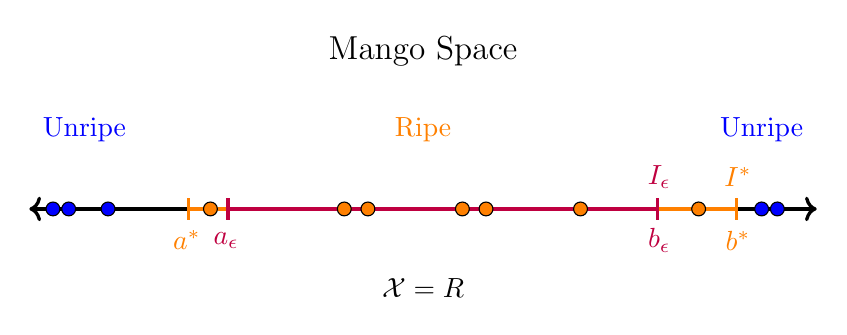
\begin{tikzpicture}
		\draw[<->,very thick] (-5,0) -- (5,0);
		\draw[color = orange, |-|,very thick] (-3,0) -- (4,0);
		\node[color=orange] at (4,.4) {$I^*$};
		\node at (0,2) {\large Mango Space} ;
		\node at (0,-1) {$\mathcal{X} = \mathbb{R}$} ;
		\node [color=blue] at (-4.3,1) {Unripe} ;
		\node [color=blue] at (4.3,1) {Unripe} ;
		\node [color=orange] at (0,1) {Ripe} ;

		\node [color=orange] at (-3,-.4) {$a^*$} ;
		\node [color=orange] at (4,-.4) {$b^*$} ;

		\draw [color=purple, |-|,very thick] (-2.5,0) -- (3,0);
		\node [color=purple] at (3,.4) {$I_\epsilon$} ;
		\node [color=purple] at (-2.5,-.4) {$a_\epsilon$} ;
		\node [color=purple] at (3,-.4) {$b_\epsilon$} ;

%		\draw [color=olive, |-|,very thick] (-3.5,0) -- (2.5,0);
%		\node [color=olive] at (3,.4) {$h_{\mathcal{T}}$} ;



		\node[circle,draw=black, fill=orange, inner sep=0pt,minimum size=5pt] at (2,0) {};
		\node[circle,draw=black, fill=orange, inner sep=0pt,minimum size=5pt] at (-1,0) {};
		\node[circle,draw=black, fill=orange, inner sep=0pt,minimum size=5pt] at (-.7,0) {};
		\node[circle,draw=black, fill=orange, inner sep=0pt,minimum size=5pt] at (.5,0) {};
		\node[circle,draw=black, fill=orange, inner sep=0pt,minimum size=5pt] at (.8,0) {};
		\node[circle,draw=black, fill=orange, inner sep=0pt,minimum size=5pt] at (-2.7,0) {};
		\node[circle,draw=black, fill=orange, inner sep=0pt,minimum size=5pt] at (3.5,0) {};

		\node[circle,draw=black, fill=blue, inner sep=0pt,minimum size=5pt] at (-4.5,0) {};
		\node[circle,draw=black, fill=blue, inner sep=0pt,minimum size=5pt] at (-4,0) {};
		\node[circle,draw=black, fill=blue, inner sep=0pt,minimum size=5pt] at (-4.7,0) {};
		\node[circle,draw=black, fill=blue, inner sep=0pt,minimum size=5pt] at (4.3,0) {};
		\node[circle,draw=black, fill=blue, inner sep=0pt,minimum size=5pt] at (4.5,0) {};
	\end{tikzpicture}
  \end{minipage}
  \vfill
  \begin{minipage}[t][0.5\textheight][t]{\textwidth}
Lets understand this visually.
$$
Err(x_0) = \sigma_\epsilon^2 + [E_\cT[\hat f(x_0)] - f(x_0)]^2 + E_\cT\big[ \hat{f}(x_0) - E_\cT[\hat{f}(x_0)] \big]^2\,.
$$\pause
Consider a data set, 
\end{minipage}
\end{frame}


\begin{frame}[fragile]{Point Variance of Linear Predictor}
Since $x_0^T  (\bfX^T\bfX)^{-1}\bfX^T\epsilon$ is a vector, squaring it is the same as multiply by its transpose. \pause This allow us to write
\begin{align*}
\action<+->{\textbf{Var} &= E_\cT\big[(\,x_0^T  (\bfX^T\bfX)^{-1}\bfX^T\epsilon\,)^2\big] && \text{From before,}}
\\
\action<+->{  &=   E_\cT\big[(\,x_0^T  (\bfX^T\bfX)^{-1}\bfX^T\epsilon\,)(\,x_0^T  (\bfX^T\bfX)^{-1}\bfX^T\epsilon\,)^T\big]  && }
\\
\action<+->{  &=   E_\cT\big[(\,x_0^T  (\bfX^T\bfX)^{-1}\bfX^T\epsilon\,)(\epsilon^T \bfX (\bfX^T\bfX)^{-1} \,x_0)\big] &&  }
\\
\action<+->{  &= (\,x_0^T  (\bfX^T\bfX)^{-1}\bfX^T) E_\cT[\epsilon\epsilon^T] (\bfX (\bfX^T\bfX)^{-1} x_0)  &&\bfX,\,x_0\,\text{const,}}
\\
\action<+->{  &=  (\,x_0^T  (\bfX^T\bfX)^{-1}\bfX^T)\,(\sigma_\epsilon^2 I)\, (\bfX (\bfX^T\bfX)^{-1} x_0)  && \text{Def. of Var,} }
\\
\action<+->{  &=  \sigma^2_\epsilon \, \,x_0^T  (\bfX^T\bfX)^{-1}x_0  && \text{Simplify.} }
\end{align*}
\action<+->{The variance is proportional to the variance in the random variable. But how do we understand the matrix $(\bfX^T\bfX)^{-1}$?}
\end{frame}


























